
$S = \{1,2,3\}$
$\Sigma = \{\emptyset, \{ 1\}, \{ 2\}, \{ 3\},  \{ 1, 2\}, \{ 2,3 \}, \{ 1,3\}, S\}$
\pagebreak
Tilfældig variabel:\\
En tilfældig variabel på $(S,\Sigma, P)$ er en funktion $X:S\to \R$ således at:\\
$\forall x\in \R : \{s \in S: X(s)\leq x\} \in \Sigma$

Tilfældig diskret variabel:\\
Billedet er en tællelig delmængde af $\R$\\
$\forall x\in \R : \{s \in S: X(s) = x\} \in \Sigma$


\begin{minipage}\textwidth
\begin{defn}\textbf{Hændelsesrum}\\
    Lad $S$ være et udfaldsrum for et eksperiment $\E$.
    
    Hændelsesrummet er givet ved potensmængden
    $\Sigma = \{A:A\subseteq S\}$.
\end{defn}
\end{minipage}
derved er hændelsesmængden givet ud fra alle mulige hændelser

\begin{minipage}\textwidth
\begin{defn}\textbf{Sandsynlighedsrum}\\
    Lad $S$ være et udfaldsrum, $A$ et hændelsesrum til $S$ og $P$ et sandsynlighedsmål over hændelsesrummet. 
    
    Så er sandsynlighedsrummet givet ved tretupelen $(S, \Sigma, P)$ for et eksperiment, $\E$.
\end{defn}
\end{minipage}


% \begin{minipage}\textwidth
% \begin{defn}\textbf{Tilfældig variabel} %Ny definition
% \newline
% En tilfældig variabel er en variabel, $x\in \R$, der får sin værdi fra et tilfældigt eksperiment.
% \end{defn}
% \end{minipage}

% \begin{minipage}\textwidth
% \begin{defn}\textbf{Tilfældig variabel} %Ny definition
% \newline
% Lad $\E$ være et eksperiment med sandsynlighedsrummet $(S, \Sigma, P)$.

% Så er en tilfældig variabel en funktion på sandsynlighedsrummet $X:S\to \R$.


% \end{defn}
% \end{minipage}


En tilfældig variabel, $X$, er en reel variabel som får sin værdi fra et eksperiment. 
Tilfældige variabler kan udtrykkes som reelle funktioner, der tildeler reelle værdier til de mulige udfald af eksperimentet.

%En tilfældig variabel er en variabel, $X$, der først tildeles en værdi efter eksperimentet er udført. 
Da $X$ først antager en værdi efter eksperimentet, er det kun muligt at beskrive billedet af $X$, som er mængden af mulige værdier $X$ kan antage, samt de  tilhørende sandsynligheder. Billedet af $X$ betegnes $range(X)$ og de tilhørende sandsynligheder kaldes for \textit{fordelingen} af $X$.

% Før eksperimentet er det muligt at beskrive mængden af mulige værdier, $range(X)$, og de tilhørende sandsynligheder, \textit{fordelingen} af $X$.
% Det betyder, at det er muligt at beskrive billedet af $X$, men ikke hvilken værdi $X$ antager.

\begin{minipage}\textwidth
\begin{defn}\label{def:Diskret_tilfældig_variabel}\textbf{Diskret tilfældig variabel} %Ny definition
\newline
Lad $(S, \Sigma, P)$ være et sandsynlighedsrum. En diskret tilfældig variabel $X$ er en reel funktion på sandsynlighedsrummet $X:S\to \R$ således, at
%
\begin{align}
    &\text{$Range(X)$ er en tællelig delmængde af $\R$ } \quad \text{og}\label{eq:def_diskretitet_betingelsen}\\
    &\forall x\in \R: \{s\in S: X(s)=x\}\in % S\cup \{\emptyset\} \subseteq 
    \Sigma\label{eq:def_tilfældig_variabel}
\end{align}

\end{defn}
\end{minipage}


At en funktion er diskret betyder, at dens billede er tællelig. 
I \autoref{def:Diskret_tilfældig_variabel} er
\eqref{eq:def_diskretitet_betingelsen} betingelsen, der sikrer, at $X$ er en diskret funktion.

%Dette betyder, at \eqref{eq:def_diskretitet_betingelsen} er betingelsen, der sikrer, at $X$ er diskret.  


% Betingelse (2,2):\\ 
% Da den værdi en diskret variabel $X$ antager, ikke kan forudsiges, 



% En diskret variabel $X$ antager værdier fra $\R$, men man kan ikke forudsige værdien af $X$ før eksperimentet er udført.

% Af denne grund, vil vi finde sandsynligheden for at $X$ er en given værdi $x$. 

%Det bemærkes, at $X$ antager værdien $x$ hvis og kun hvis resultatet af eksperimentet ligger i delmængden som afbilledes over i $x$ - altså delmængden $X^{-1}(x) = \{s\in S: X(s)=x\}$. Betingelse (2,2) postulerer at alle sådanne delmængder er hændelser, og da alle kombinationer af hændelser er i $\Sigma$, kan en tilsvarende sandsynlighed findes.

Det bemærkes, at $X$ antager værdien $x$ hvis og kun hvis resultatet af eksperimentet, $\E$, ligger i en delmængde af $S$ som afbilledes over i $x$. Derved ligger resultatet af $\E$ i delmængden $X^{-1}(x) = \{s\in S: X(s)=x\} \subseteq S\cup \{\emptyset\}$, hvor det bemærkes, at  $X^{-1}(x)\subseteq S\cup \{\emptyset\} \subseteq \Sigma$.
Betingelse \eqref{eq:def_tilfældig_variabel} gør derfor, at alle sådanne delmængder er elementer af hændelsesrummet, $\Sigma$, og derfor har en tilsvarende sandsynlighed, $P$.

Da den diskret tilfældige variabel kan antage flere værdier, defineres en funktion, der bestemmer sandsynligheden for hvert udfald af den diskret tilfældige variabel.

Fremadrettet vil $\{s\in S: X(s)=x\}$ blive betegnet $\{X=x\}$.

\begin{minipage}\textwidth
\begin{defn}\label{def:Frekvensfunktionen}\textbf{Frekvensfunktionen} %Ny definition
\newline
    Lad $X$ være en diskret tilfældig variabel. % med range $\{x_k| k\in N \subseteq \N\}$. 
    Funktionen $p_X:\R\to [0,1]$ defineret ved
%    
    $$ p_X(x) = P(X = x)$$
%    
    kaldes for \textit{frekvensfunktionen} eller \textit{pmf} til $X$.
\end{defn}
\end{minipage}

Frekvensfunktionen er derved sandsynligheden for at afbildingen $X$ antager værdien $x$.
Hvis en hændelse ikke er element af $range(X)$ vil frekvensfunktionen give $0$. 
%$p_X(x)=0$ for $x\notin range(X)$.

\begin{minipage}\textwidth
\begin{pro}\label{prop:frekvensfunktion}\textbf{}\\
    Lad $X$ være en diskret tilfældig variabel og lad $p_X$ være den tilhørende frekvensfunktion. Så gælder det, at
    %
   % En funktion $p_X$ er en frekvensfunktion for en diskret tilfældig variable $X$, %  med $range(X)=\{x_k | k\in N \subseteq \N\}$
    %hvor det gælder, at
    \begin{enumerate}
        \item[(a)] $\displaystyle p_X(x)\geq 0$
        %\item[(b)] $\displaystyle \sum_{k=1}^\infty p(x_k)=1$
        \item[(b)] $\displaystyle \sum_{x\in \R} p_X(x)=1$
    \end{enumerate}
    %hvor summen er endelig, hvis $range(X)$ er endelig.
    for alle $x\in \R$.
\end{pro}
\end{minipage}

\begin{bev} \textbf{} %Nyt bevis
\newline
Lad $X$ være en diskret tilfældig variabel der kan antage værdier $x\in\R$ og lad $p_X(x)$ være en frekvensfunktion til $X$.
\begin{itemize}
    \item []\textbf{Bevis for punkt (a)}\\
    % Antag først at, $x\in Range(X)$, så vil frekvensfunktionen være sandsynligheden for at $X$ giver hændelsen $x$. Fra \autoref{def:sandsynlighedsregningens_grundsætninger} punkt (a) fås, at enhver hændelse har en ikke-negative sandsynlighed, og derfor må $p_X(x) = P(X=x) \geq 0$. \\
    % Antag omvendt, at $x\notin Range(X)$, så vil det være en umulig hændelse, at $X$ giver hændelsen $x$. Da sandsynligheden af en umulig hændelse altid er 0, fås $p_X(x)=P(\emptyset) = 0$.\\
    % Derved er det bevist, at $p_X(x) \geq 0$
    % 
    Da $x\in \R$, er frekvensfunktionen defineret over alle $x$ og angiver sandsynligheden for, at $X$ giver hændelsen $x$. Fra \autoref{def:sandsynlighedsregningens_grundsætninger} punkt (a) fås, at enhver hændelse har en ikke-negative sandsynlighed, og derfor må $p_X(x) = P(X=x) \geq 0$.
    Derved er det bevist, at $p_X(x) \geq 0$
    
    \item[]\textbf{Bevis for punkt (b)}\\
    Lad $ \sum_{x\in \R} p_X(x)$ være givet.
    Summen omskrives ved brug af \autoref{def:Frekvensfunktionen}.
    \begin{align*}
    \sum_{x\in \R} p_X(x) &=  \sum_{x\in \R} P(X=x)
    \intertext{Dette omskrives ved brug af  \autoref{def:sandsynlighedsregningens_grundsætninger} punkt (c)}
     \sum_{x\in \R} P(X=x)  &= P\left( \bigcup_{x\in \R} \{X=x\}\right)\\
    &= P\left( \bigcup_{x\in \R} \{s\in S: X(s)=x\}\right) \\
    &= P\left( \bigcup_{x\in Range(X)} \{s\in S: X(s)=x\}\right) + P\left( \bigcup_{x\notin Range(X)} \{s\in S: X(s)=x\}\right)\\
     %P\left( S\cup \emptyset \right) = P(S) + P(\emptyset) 
    &= P(S) + P(\emptyset)
\end{align*} 
    Fra \autoref{def:sandsynlighedsregningens_grundsætninger} punkt (b) gælder det, at $P(S)=1$ og $P(\emptyset)=0$. Det er dermed bevist, at $\displaystyle \sum_{x\in \R} p_X(x)=1$.
\end{itemize}
\end{bev}

Hvis frekvensfunktionen har den samme værdi for alle de mulige udfald er det en uniform fordeling. \\
Frekvensfunktionen kan illustreres i et pindediagram, hvor søjlerne er de forskellige udfald, og højden af en given søjle repræsenterer sandsynligheden for udfaldet.
\textbf{overvej eksempel der viser pindediagram/sim}

\begin{eks} \textbf{} %Nyt eksempel
\newline
I et eksperiment $\E$ kastes to fair terninger. \\ $S=\left\{\{1,1\},\{1,2\},\cdots,\{6,6\}\right\}$ hvor $|S|=6^2 = 36$
%$S = \{2, 3, 4, 5, 6, 7, 8, 9, 10, 11, 12\},$
Lad $X$ være summen af de to terningkast og lad $X$ være givet således, at $Range(X)=\{2, 3, 4, 5, 6, 7, 8, 9, 10, 11, 12\}$.
Sandsynlighederne for at ${X=x}$ kan findes med frekvensfunktionen, hvor  $p_X(2)=\frac{1}{36}, p_X(3)=\frac{2}{36}, \cdots, p_X(12)=\frac{1}{36}$ 


    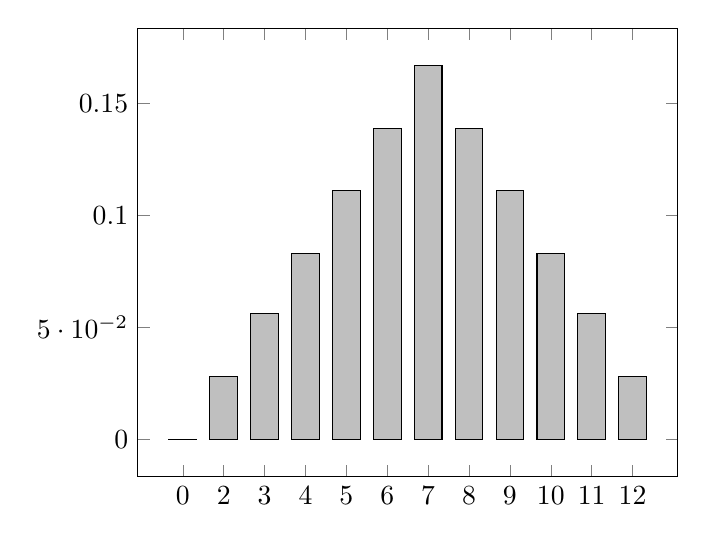
\begin{tikzpicture}
        \begin{axis}[
            symbolic x coords={0, 2, 3, 4, 5, 6, 7, 8, 9, 10, 11, 12},
            xtick=data
          ]
            \addplot[ybar,fill=lightgray] coordinates {
                (0, 0.0000001)
                (2, 0.028)
                (3,  0.056)
                (4,   0.083)
                (5,   0.111)
                (6,  0.139)
                (7,   0.167)
                (8,   0.139)
                (9,  0.111)
                (10,   0.083)
                (11,   0.056)
                (12,  0.028)
            };
        \end{axis}
    \end{tikzpicture}
    

\begin{tikzpicture}
\begin{axis}
\addplot+[ycomb, color=black] plot coordinates
	{(0,3) (1,2) (2,4) (3,1) (4,2)};
\end{axis}
\end{tikzpicture}

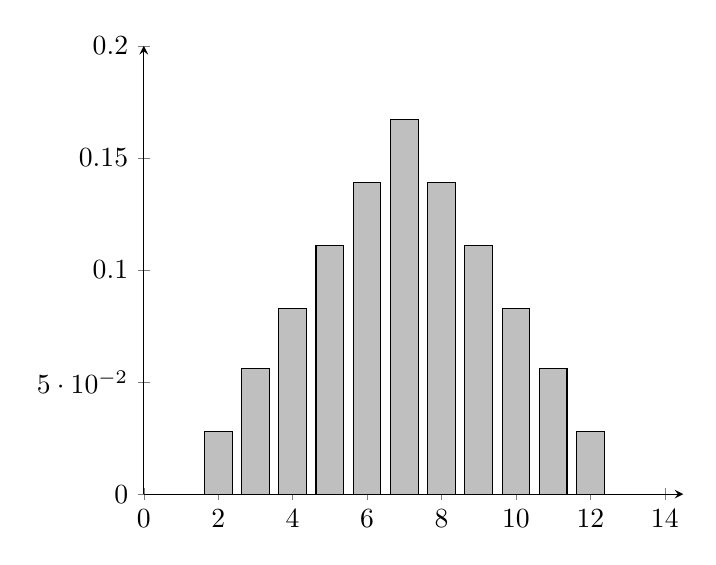
\begin{tikzpicture}
\begin{axis}[axis x line=bottom,
	axis y line=left, ymax=0.2, ymin=0, xmax=14.5, xmin=0]
\addplot [ybar, color=black, fill=lightgray] coordinates
	{           (0, 0)
	            (1, 0)
                (2, 0.028)
                (3,  0.056)
                (4,   0.083)
                (5,   0.111)
                (6,  0.139)
                (7,   0.167)
                (8,   0.139)
                (9,  0.111)
                (10,   0.083)
                (11,   0.056)
                (12,  0.028)}
                (13, 0)
                (14, 0);
\end{axis}
\end{tikzpicture}

% \begin{align*}
%     % p_X(2)=\frac{1}{36}; \quad  p_X(3)=\frac{2}{36}; \quad p_X(4)=\frac{3}{36}; \quad  p_X(5)=\frac{4}{36}; \quad
%     % p_X(6)=\frac{5}{36}\\
%     % p_X(7)=\frac{6}{36}\\
%     % p_X(8)=\frac{5}{36}\\
%     % p_X(9)=\frac{4}{36}\\
%     % p_X(10)=\frac{3}{36}\\
%     % p_X(11)=\frac{2}{36}\\
%     % p_X(12)=\frac{1}{36}\\
% \end{align*}

\end{eks}

%$\Sigma = {{}, {1}, {2}, {3}, {4}, {5}, {6}, {1, 2}, {1, 3}, {1, 4}, {1, 5}, {1, 6}, {2, 3}, {2, 4}, {2, 5}, {2, 6}, {3, 4}, {3, 5}, {3, 6}, {4, 5}, {4, 6}, {5, 6}, {1, 2, 3}, {1, 2, 4}, {1, 2, 5}, {1, 2, 6}, {1, 3, 4}, {1, 3, 5}, {1, 3, 6}, {1, 4, 5}, {1, 4, 6}, {1, 5, 6}, {2, 3, 4}, {2, 3, 5}, {2, 3, 6}, {2, 4, 5}, {2, 4, 6}, {2, 5, 6}, {3, 4, 5}, {3, 4, 6}, {3, 5, 6}, {4, 5, 6}, {1, 2, 3, 4}, {1, 2, 3, 5}, {1, 2, 3, 6}, {1, 2, 4, 5}, {1, 2, 4, 6}, {1, 2, 5, 6}, {1, 3, 4, 5}, {1, 3, 4, 6}, {1, 3, 5, 6}, {1, 4, 5, 6}, {2, 3, 4, 5}, {2, 3, 4, 6}, {2, 3, 5, 6}, {2, 4, 5, 6}, {3, 4, 5, 6}, {1, 2, 3, 4, 5}, {1, 2, 3, 4, 6}, {1, 2, 3, 5, 6}, {1, 2, 4, 5, 6}, {1, 3, 4, 5, 6}, {2, 3, 4, 5, 6}, {1, 2, 3, 4, 5, 6}}$

\textit{Indtil videre} har hændelsen været på formen $\{X=k\}$, hvor $X$ har antaget én bestemt værdi, $k$. Dette kan udvides til hændelser på formen $\{X\leq k\}$, hvor $X$ antager værdier mindre eller lig $k$. Dette kan defineres som følgende funktion

\begin{minipage}\textwidth
\begin{defn}\textbf{Kumulative fordelingsfunktion} %Ny definition
\newline
Lad $X$ være en tilfældig variabel. Funktionen 
$$F(x)=P(X\leq x), \quad x\in\R$$
kaldes for den kumulative fordelingsfunktion (cdf) af $X$
\end{defn}
\end{minipage}

%A real random variable is a real valued function from the possible outcome of a random experiment.

\begin{minipage}\textwidth
\begin{pro} \textbf{} %Ny proposition
\newline
Lad $X$ være en diskret tilfældig variabel med $range(X)=\{x_k | k\in N \subseteq \N\}$, frekvensfunktion, $p$, og kumulative fordelingsfunktion, $F$. Så gælder det, at
\begin{enumerate}
    \item $\displaystyle F(x)=\displaystyle\sum_{k:x_k\leq x}p(x_k), \quad x\in\R$
    \item $\displaystyle p(x_k)=F(x_k)-\lim_{y\uparrow x_k} F(y), \quad k=1, 2,\cdots$
    \item For $B\subseteq \R$, $\displaystyle P(X\in B)=\displaystyle\sum_{k:x_k\in B}p(x_k)$
\end{enumerate}
\end{pro}
\end{minipage}